%\definecolor{BLUE_Color}{RGB}{171, 216, 231}
\definecolor{BLUE_Color}{RGB}{255, 255, 255}
\definecolor{ORANGE_Color}{RGB}{249, 164, 27}

\usetikzlibrary{shadows}
\usetikzlibrary{automata, positioning, arrows, calc}
      \definecolor{falured}{rgb}{0.5, 0.09, 0.09}
     \newcommand{\fmbtsymbex}[1]{\textcolor{falured}{ #1}}
     \newcommand{\fmbtsymbexReg}[1]{ \textcolor{falured}{ #1} }
     \definecolor{mycolorData}{rgb}{0.07, 0.04, 0.56}


      \definecolor{mycolorF}{rgb}{0.973, 0.882, 0.882} 
     \definecolor{mycolorP}{rgb}{0.902, 0.957, 0.918}
     \definecolor{mycolorI}{rgb}{1.000, 0.969, 0.800}


\tikzset{
	%->,  % makes the edges directed
	%>=stealth, 
	% makes the arrow heads bold
	shorten >=2pt, shorten <=2pt, % shorten the arrow
	node distance=3cm, % specifies the minimum distance between two nodes. Change if n
	every state/.style={draw=blue!55,very thick,fill=blue!20}, % sets the properties for each ’state’ n
	initial text=$ $, % sets the text that appears on the start arrow
	%node distance=2.5cm,
    %every edge/.style={draw, bend left=20, ->}
    circled node/.style={rectangle,draw, inner sep=0, minimum size=1.5em},
    better circled node/.style={circled node,text height=.8em,text depth=.25em},
    }
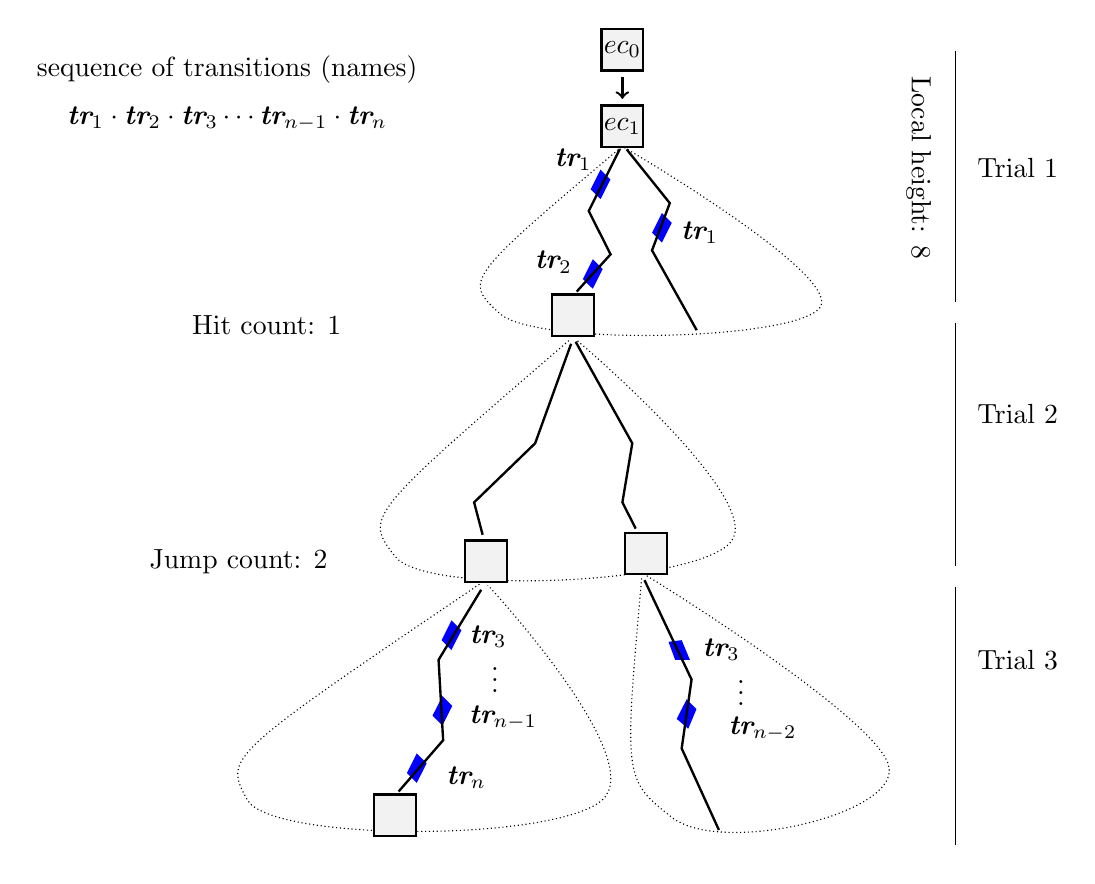
\begin{tikzpicture}
    [xscale=1.255, yscale=1.25%,font=\small %footnotesize
    ] 

\draw[densely dotted,fill=BLUE_Color]  plot[smooth, tension=.7] coordinates {(0.1194,2.82) (-1.2428,1.02) (2,1.08) (-0.0398,2.74)};
\draw[densely dotted,fill=BLUE_Color]  plot[smooth, tension=.7] coordinates {(-0.5,0.78) (-2.3,-1.4499) (1.1,-1.3) (-0.5,0.78)};
\draw[densely dotted,fill=BLUE_Color]  plot[smooth, tension=.7] coordinates {(-1.4,-1.7) (-3.7975,-3.92) (-0.2,-3.92) (-1.4,-1.7)};
\draw[densely dotted,fill=BLUE_Color]  plot[smooth, tension=.7] coordinates {(0.2,-1.6165) (0.5,-4.1) (2.7,-3.6) (0.2,-1.6165)};

\draw[fill=blue,draw=none] (-0.2214,2.48) node[scale=0.1] (v1) {} -- (-0.1214,2.38) -- (-0.2214,2.18) -- (-0.3214,2.28) -- (v1);
\draw[fill=blue,draw=none] (-0.2996,1.57) node[scale=0.1] (v12) {} -- (-0.1996,1.47) -- (-0.2996,1.27) -- (-0.3996,1.37) -- (v12);

\draw[fill=blue,draw=none] (0.4,2.04) node[scale=0.1] (v13) {} -- (0.5,1.94) -- (0.4,1.74) -- (0.3,1.84) -- (v13);

\draw[fill=blue,draw=none] (-1.7295,-2.1) node[scale=0.1] (v14) {} -- (-1.6295,-2.2) -- (-1.7297,-2.4) -- (-1.8295,-2.3) -- (v14);

\draw[fill=blue,draw=none] (-2.0806,-3.4501) node[scale=0.1] (v15) {} -- (-1.9806,-3.5501) -- (-2.0806,-3.7501) -- (-2.1806,-3.6501) -- (v15);

\draw[fill=blue,draw=none] (-1.8212,-2.867) node[scale=0.1] (v16) {} -- (-1.7212,-2.967) -- (-1.8212,-3.167) -- (-1.9212,-3.067) -- (v16);

\draw[fill=blue,draw=none] (0.6499,-2.9) node[scale=0.1] (v17) {} -- (0.7499,-3) -- (0.6666,-3.2) -- (0.5499,-3.1) -- (v17);


\draw[fill=blue,draw=none] (0.4666,-2.3167) node[scale=0.1] (v33) {} -- (0.6,-2.3) -- (0.6833,-2.5) -- (0.5334,-2.5) -- (v33);

\draw[ line width=.3mm] (0,2.74) node[scale=0.1] (v2) {} -- (-0.3408,2.06) -- (-0.1194,1.62) -- (-0.5,1.2);


\node at (-0.5,2.58) {$\textbf{\em tr}_1$};
\node at (-0.699,1.54) {$\textbf{\em tr}_2$};
\draw[ line width=.3mm] (v2) -- (0.4796,2.14) -- (0.3,1.66) -- (0.7796,0.8);
\node at (0.7806,1.84) {$\textbf{\em tr}_1$};

\draw[ line width=.3mm]  (-0.5,0.7639) -- (-0.8829,-0.3) -- (-1.5006,-0.9) -- (-1.4,-1.2835);

\draw[ line width=.3mm] (-0.5002,0.7808) -- (0.1,-0.3) -- (0,-0.9) -- (0.1604,-1.2169);
\draw[ line width=.3mm] (0.2,-1.64) -- (0.7,-2.7) -- (0.6,-3.4) -- (1,-4.28);
\draw[ line width=.3mm] (-1.4,-1.74) -- (-1.8602,-2.5) -- (-1.814,-3.3169) -- (-2.301,-3.88);
\node at (-1.3594,-2.2631) {$\textbf{\em tr}_3$};
\node at (1,-2.4) {$\textbf{\em tr}_3$};
\node at (-1.2066,-3.087) {$\textbf{\em tr}_{n-1}$};
\node at (-1.5804,-3.7) {$\textbf{\em tr}_n$};
\node at (1.4175,-3.2) {$\textbf{\em tr}_{n-2}$};
\node[circled node,line width=.3mm,fill=gray!10] (v3) at (0,3.7) {$ec_0$};
\node[circled node,line width=.3mm,fill=gray!10] (v4) at (0,2.92) {$ec_1$};
\node[circled node,line width=.3mm,fill=gray!10] at (-2.301,-4.08) {$$};
\node[circled node,line width=.3mm,fill=gray!10] at (-1.3806,-1.5) {};
\node[circled node,line width=.3mm,fill=gray!10] at (0.2388,-1.42) {};
\node[circled node,line width=.3mm,fill=gray!10] at (-0.5,1) {};
\draw (3.3678,-4.44) -- (3.3678,-1.7);
\draw (3.3678,1.08) -- (3.3678,3.74);
\draw (3.3678,-1.6) -- (3.3678,0.98);
\node[rotate=-90] at (3,2.5) {Local height: 8};
\node at (-3.6,0.9) {Hit count: 1};
\node at (-3.8839,-1.5) {Jump count: 2};
\node at (4,2.5) {Trial 1};
\node at (4,-2.5) {Trial 3};
\node at (4,0) {Trial 2};
\node at (-1.2901,-2.6202) {\vdots};
\node at (1.2,-2.7501) {\vdots};
\node at (-4,3) {$\textbf{\em tr}_1 \cdot \textbf{\em tr}_2 \cdot \textbf{\em tr}_3 \cdots \textbf{\em tr}_{n-1} \cdot\textbf{\em tr}_{n}$};

\node at (-4,3.5) { sequence of transitions (names)};
\draw[ line width=.3mm, -> ]   (v3) edge (v4);
\end{tikzpicture}